\documentclass[10pt,twocolumn]{article}

% ---- Packages (all standard on Overleaf; compiles out of the box) ----
\usepackage[utf8]{inputenc}
\usepackage[T1]{fontenc}
\usepackage{lmodern}
\usepackage[margin=1in]{geometry}
\usepackage{amsmath,amssymb}
\usepackage{booktabs}
\usepackage{graphicx}
\usepackage{xcolor}
\usepackage{tikz}
\usetikzlibrary{arrows.meta,positioning}
\usepackage{authblk}
\usepackage[colorlinks=true,linkcolor=black,citecolor=black,urlcolor=blue]{hyperref}

\title{\textbf{A Confidence You Can Measure:\\ Validating Confidence-Gated Authorization for AI Agents}}

\author[1]{Abenezer Getachew}
\affil[1]{Lelu \quad \texttt{abenezergetachew1990@gmail.com}}
\date{}

\begin{document}
\maketitle

\begin{abstract}
Authorization systems for AI agents increasingly propose gating actions on
\emph{model confidence}: allow a tool call when the model is confident, and
escalate to a human, downgrade scope, or deny when it is not. This design rests
on a single untested premise---that low confidence predicts wrong or unsafe
actions. If the premise is false, a confidence gate stops a random subset of
actions and gives operators a false sense of safety. We make three
contributions. First, we describe the confidence gate implemented in Lelu, an
open-source authorization engine, including logprob-based score extraction and an
isotonic-regression calibrator. Second, we define a reproducible benchmark that
scores the premise directly with the area under the ROC curve (AUROC) of
\emph{confidence $\rightarrow$ correctness}. Third, we report evidence on
$321{,}105$ real answers from $15$ chat models across five multiple-choice
benchmarks, drawn from published model outputs: overall AUROC is $0.709$ and
reaches $0.83$ on the strongest models (GPT-4o), clearing a ``strong signal''
threshold precisely on the capable models such a gate would target. We are
explicit about what this does and does not establish---it is multiple-choice
question answering, not agent tool-calls, and correctness is a proxy for
safety---and we release the code and an agent-action benchmark scaffold
(BFCL, $\tau$-bench) as the next milestone.
\end{abstract}

\section{Introduction}
Traditional authorization tools---policy engines such as OPA and Casbin, or cloud
services such as AWS Verified Permissions---answer \emph{who may do what}. They
block unauthorized access, but they cannot detect when a \emph{legitimately
authorized} agent is being manipulated (through prompt injection, an
out-of-distribution request, or a low-confidence decision) into taking a
dangerous action. As LLM agents are given real tools---issuing refunds, deleting
records, sending messages---this gap becomes a security problem.

A natural proposal is to gate each action on the model's own confidence. Lelu
implements exactly this: a per-action confidence score is compared against
thresholds that map to four outcomes---full permission, human review, a downgrade
to read-only scope, or a hard deny. The appeal is that confidence is a
model-agnostic, always-available signal.

The entire design, however, depends on one sentence being true:
\begin{quote}
\emph{When the model is less confident, the action is more likely to be wrong or
unsafe.}
\end{quote}
If that sentence holds, watching confidence is a principled way to catch bad
actions. If it does not---if confident actions are just as likely to be wrong as
unsure ones---then a low-confidence gate blocks a random subset of actions,
stopping some real mistakes while waving confident mistakes through, and offering
operators unwarranted assurance. \emph{A confidence gate you cannot measure is
theater.} Our aim is to measure it.

We treat the premise as an empirical claim and score it with a single number, the
AUROC of confidence against correctness (Section~\ref{sec:method}). Because
running live agents at scale is expensive, we first obtain a lower-bound estimate
from a large corpus of \emph{published} model outputs on multiple-choice question
answering (Section~\ref{sec:results}), then release a scaffold for the harder,
agent-action version of the same measurement.

\section{Background and Related Work}
\paragraph{Agent authorization and guardrails.}
Policy engines (OPA, Casbin) and permission services (AWS Verified Permissions)
enforce access control but are confidence-agnostic. Guardrail and safety layers
add content filters and human-in-the-loop review. Confidence-based gating is
complementary: it targets the case where an authorized action is nonetheless
untrustworthy.

\paragraph{Confidence and calibration.}
Softmax probabilities are a cheap confidence signal but are known to be
miscalibrated in modern networks~\cite{guo2017calibration}. Post-hoc methods
recover calibration: temperature scaling~\cite{guo2017calibration} and isotonic
regression~\cite{niculescu2005predicting}. Crucially, calibration (whether a
reported $0.8$ means $80\%$) is distinct from \emph{ranking} (whether more
confident actions are more often correct); gating needs the latter, which can
hold even when the former fails~\cite{plaut2025probabilities}.

\paragraph{Stronger confidence signals.}
Beyond single-pass logprobs, self-consistency across samples~\cite{wang2022self}
and semantic-entropy scoring~\cite{kuhn2023semantic,farquhar2024detecting}
provide stronger, if costlier, uncertainty estimates. Conformal
prediction~\cite{angelopoulos2021gentle} offers distribution-free guarantees and
is a natural research direction for turning a heuristic score into a bound.

\paragraph{Agent benchmarks.}
The Berkeley Function-Calling Leaderboard (BFCL)~\cite{patil2023gorilla} provides
per-example gold tool calls, enabling deterministic per-action labels;
$\tau$-bench~\cite{yao2024taubench} and TheAgentCompany~\cite{xu2024agentcompany}
provide realistic multi-turn tasks. These are the settings our agent-action
benchmark targets.

\section{The Confidence Gate}
Lelu's gate has three stages, mirrored by the released implementation.

\paragraph{Score extraction.}
For providers that expose token-level signals, a raw score $s\in[0,1]$ is derived
from token logprobs or probabilities (or, for local models, normalized entropy).
When a model exposes no such signal (for example, some hosted Claude endpoints),
the system \emph{declines to fabricate one} and defers to an explicit
missing-signal policy rather than inventing a number.

\paragraph{Calibration.}
An isotonic-regression calibrator~\cite{niculescu2005predicting} maps raw scores
to calibrated threat probabilities using the pool-adjacent-violators algorithm,
fitted online from human-review outcomes, with a feedback-tuned decision
threshold. Isotonic regression is non-parametric and enforces monotonicity
(higher raw score $\rightarrow$ higher calibrated probability), which is what a
gate requires.

\paragraph{Gating.}
A calibrated score $c$ is compared to policy thresholds, yielding one of four
outcomes:
\[
\text{outcome}(c)=
\begin{cases}
\text{full permission} & c \ge 0.90\\
\text{human review} & 0.70 \le c < 0.90\\
\text{read-only} & 0.50 \le c < 0.70\\
\text{hard deny} & c < 0.50
\end{cases}
\]
Thresholds are overridable per policy. Figure~\ref{fig:pipeline} shows the flow.

\begin{figure}[t]
\centering
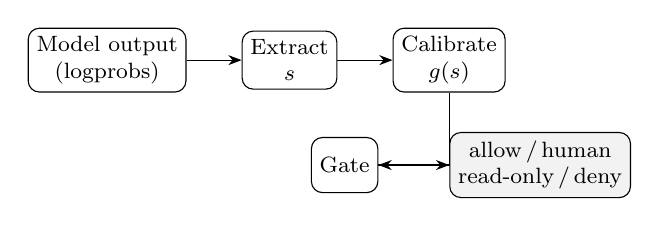
\begin{tikzpicture}[
  node distance=6mm and 7mm,
  box/.style={draw, rounded corners, align=center, font=\footnotesize,
              minimum height=7mm, inner sep=3pt},
  >={Stealth[]}]
\node[box] (m) {Model output\\(logprobs)};
\node[box, right=of m] (e) {Extract\\$s$};
\node[box, right=of e] (c) {Calibrate\\$g(s)$};
\node[box, below=of e, xshift=7mm] (g) {Gate};
\node[box, right=of g, xshift=2mm, fill=black!5] (o)
  {allow\,/\,human\\read-only\,/\,deny};
\draw[->] (m) -- (e);
\draw[->] (e) -- (c);
\draw[->] (c.south) |- (g.east);
\draw[->] (g) -- (o);
\end{tikzpicture}
\caption{The confidence gate: a raw score $s$ is extracted from model output,
calibrated to $g(s)$, and compared against policy thresholds to select an
authorization outcome.}
\label{fig:pipeline}
\end{figure}

\section{Validation Benchmark}
\label{sec:method}
The benchmark answers one question: \emph{does confidence separate correct actions
from wrong ones?} It reduces to two columns---a confidence value and a binary
correctness label per action---and a single score over them.

\paragraph{Metric.}
Let $c_i$ be the confidence of action $i$ and $y_i\in\{0,1\}$ its correctness
($1=$ correct). The AUROC of confidence predicting correctness is the probability
that a randomly chosen correct action has higher confidence than a randomly chosen
wrong one,
\begin{equation}
\mathrm{AUROC} = \Pr\big(c_i > c_j \mid y_i=1,\, y_j=0\big),
\end{equation}
estimated with the rank (Mann--Whitney) statistic. We interpret it against a
fixed rubric: $\ge 0.75$ strong (build it); $0.65$--$0.75$ promising;
$0.55$--$0.65$ weak; ${\approx}0.50$ no signal. We also report the
\emph{confident-wrong rate}---the fraction of wrong actions above the gate
threshold---as an explicit measure of the blind spot.

\paragraph{Confidence signals.}
Three measures are supported: (i) mean token probability from logprobs (cheapest,
one call); (ii) self-consistency, the fraction of $n$ samples agreeing on the
modal action~\cite{wang2022self}; and (iii) verbalized confidence, used only as a
weak baseline. We expect self-consistency to dominate logprobs.

\paragraph{Labeling.}
Per-action labels require a gold action. We therefore begin with
BFCL~\cite{patil2023gorilla}, where $\text{wrong}=(\text{predicted call}\neq
\text{gold call})$ is deterministic, and graduate to
$\tau$-bench~\cite{yao2024taubench} for realistic unsafe-action cases.
Task-level success labels are too coarse for an action gate and are avoided.

\paragraph{Evidence-layer proxy.}
Running many models live is costly, so we first estimate a \emph{lower bound} on
the premise from published model outputs on multiple-choice question answering
(Section~\ref{sec:results}). Here confidence is the maximum softmax probability
and $y_i$ is answer correctness. This is the cheapest signal on the tidiest
setting, so it under-estimates what stronger signals on curated actions would
yield.

\section{Results}
\label{sec:results}
We reuse the released per-question outputs of Plaut et
al.~\cite{plaut2025probabilities}: $321{,}105$ answers from $15$ chat models
across ARC, HellaSwag, MMLU, TruthfulQA, and WinoGrande. For each answer we take
confidence $=\max$ softmax probability and whether it was correct, and compute
AUROC. No model inference or API key is required; the computation is a rank
statistic over the published files.

\begin{table}[t]
\centering
\caption{AUROC of confidence $\rightarrow$ correctness, per model
($n=21{,}407$ each). Confidence is the maximum softmax probability.}
\label{tab:models}
\small
\begin{tabular}{lcc}
\toprule
Model & Accuracy & AUROC \\
\midrule
GPT-4o        & 0.860 & \textbf{0.830} \\
Llama3.1-70b  & 0.802 & 0.821 \\
Llama3-70b    & 0.781 & 0.793 \\
GPT-3.5-turbo & 0.675 & 0.756 \\
Llama3.1-8b   & 0.612 & 0.716 \\
Yi-34b        & 0.688 & 0.710 \\
Llama3-8b     & 0.609 & 0.707 \\
Yi-6b         & 0.500 & 0.652 \\
Falcon-40b    & 0.415 & 0.640 \\
Solar         & 0.685 & 0.627 \\
Llama2-70b    & 0.592 & 0.615 \\
Falcon-7b     & 0.325 & 0.613 \\
Mistral       & 0.552 & 0.590 \\
Llama2-7b     & 0.436 & 0.574 \\
Mixtral       & 0.680 & 0.569 \\
\bottomrule
\end{tabular}
\end{table}

\begin{table}[t]
\centering
\caption{AUROC by task (pooled over all $15$ models).}
\label{tab:tasks}
\small
\begin{tabular}{lcc}
\toprule
Task & Accuracy & AUROC \\
\midrule
ARC        & 0.730 & 0.800 \\
HellaSwag  & 0.612 & 0.738 \\
TruthfulQA & 0.524 & 0.731 \\
MMLU       & 0.579 & 0.729 \\
WinoGrande & 0.614 & 0.601 \\
\bottomrule
\end{tabular}
\end{table}

The pooled AUROC is $\mathbf{0.709}$ (accuracy $0.614$). Table~\ref{tab:models}
gives the per-model breakdown and Table~\ref{tab:tasks} the per-task breakdown.
Three findings stand out.

\paragraph{The premise survives contact with real data.}
Confidence predicts correctness above chance for every model and task, and on the
strongest models (GPT-4o $0.830$, Llama3.1-70b $0.821$) it clears the ``strong
signal'' bar---using only the cheapest confidence measure.

\paragraph{The signal is conditional.}
Weak models (Mixtral $0.569$, Mistral $0.590$) and one hard task
(WinoGrande $0.601$) fall toward ``weak.'' A confidence gate should therefore
target capable models and report its reliability per model rather than assume it
holds universally.

\paragraph{Stronger models rank better.}
The most capable, most heavily aligned models had the \emph{best} AUROC. While
alignment is known to hurt absolute calibration, the \emph{ranking} that a gate
depends on is preserved on strong models---a point in favor of the design.

\section{Discussion: What This Does and Does Not Prove}
We are deliberate about the limits, because honest failure reporting is the point.
\begin{enumerate}
\item \textbf{Cheapest signal.} Maximum softmax is the weak baseline; the
literature and our design expect self-consistency and semantic
entropy~\cite{wang2022self,farquhar2024detecting} to exceed it. The reported
$0.71$--$0.83$ is thus closer to a floor than a ceiling.
\item \textbf{Q\&A, not tool-calls.} Confidence over four clean options is tidier
than confidence over generated tool arguments. This is an optimistic proxy for the
agent setting, not a measurement of it.
\item \textbf{Correctness is not safety.} Lelu gates unsafe actions; correctness
is a related but distinct target.
\end{enumerate}
Limits (2) and (3) are exactly what the released agent-action benchmark
addresses. It ships a runnable demonstration (synthetic ``signal'' versus
``noise'' worlds) and a scaffold requiring only a dataset loader and a model
sampler to produce a real AUROC on BFCL or $\tau$-bench.

\section{Roadmap}
The evidence licenses continued work in a specific shape. \emph{Available now:}
logprob-based extraction, four-outcome gating, isotonic calibration with a
feedback loop, and human-in-the-loop review. \emph{Next:} temperature scaling on
held-out data so reported confidence is numerically calibrated; self-consistency
and semantic-entropy signals for high-stakes actions. \emph{Research track:}
conformal guarantees~\cite{angelopoulos2021gentle} that emit calibrated reliable
sets rather than point scores, and calibration in low-resource languages and
underrepresented domains, where confidence is least reliable and existing
guardrail platforms are silent.

\section{Conclusion}
Confidence-gated authorization is only as good as the premise that low confidence
predicts bad actions. We measured that premise on $321{,}105$ real answers and
found it holds---strongly on capable models (AUROC up to $0.83$), conditionally
elsewhere---using the weakest available signal. This is genuine, independent
support for building the \emph{rigorous} version of a confidence gate, while the
agent-action benchmark remains the decisive next measurement. The value of
publishing the number, the per-model variation, and the blind spots is precisely
that it turns a claim into something an operator can trust.

\section*{Reproducibility}
The benchmark code, the exact per-model and per-task results, and the
agent-action scaffold are released in the project repository under
\texttt{benchmark/}. The evidence-layer result is reproduced with
\texttt{python benchmark/confidence\_auroc.py}, which uses only \texttt{numpy}
(AUROC via the rank formula) and the published dataset
of~\cite{plaut2025probabilities}.

\begin{thebibliography}{99}
\small
\bibitem{guo2017calibration}
C.~Guo, G.~Pleiss, Y.~Sun, and K.~Q. Weinberger.
On calibration of modern neural networks.
\emph{ICML}, 2017.

\bibitem{niculescu2005predicting}
A.~Niculescu-Mizil and R.~Caruana.
Predicting good probabilities with supervised learning.
\emph{ICML}, 2005.

\bibitem{plaut2025probabilities}
B.~Plaut et al.
Probabilities of chat LLMs are miscalibrated but still predict correctness on
multiple-choice Q\&A.
\emph{TMLR}, 2025.

\bibitem{wang2022self}
X.~Wang et al.
Self-consistency improves chain-of-thought reasoning in language models.
\emph{ICLR}, 2023.

\bibitem{kuhn2023semantic}
L.~Kuhn, Y.~Gal, and S.~Farquhar.
Semantic uncertainty: Linguistic invariances for uncertainty estimation in
natural language generation.
\emph{ICLR}, 2023.

\bibitem{farquhar2024detecting}
S.~Farquhar, J.~Kossen, L.~Kuhn, and Y.~Gal.
Detecting hallucinations in large language models using semantic entropy.
\emph{Nature}, 630:625--630, 2024.

\bibitem{angelopoulos2021gentle}
A.~N. Angelopoulos and S.~Bates.
A gentle introduction to conformal prediction and distribution-free uncertainty
quantification.
\emph{arXiv:2107.07511}, 2021.

\bibitem{patil2023gorilla}
S.~G. Patil, T.~Zhang, X.~Wang, and J.~E. Gonzalez.
Gorilla: Large language model connected with massive APIs.
\emph{NeurIPS}, 2024. (Berkeley Function-Calling Leaderboard.)

\bibitem{yao2024taubench}
S.~Yao, N.~Shinn, P.~Razavi, and K.~Narasimhan.
$\tau$-bench: A benchmark for tool-agent-user interaction in real-world domains.
\emph{arXiv:2406.12045}, 2024.

\bibitem{xu2024agentcompany}
F.~F. Xu et al.
TheAgentCompany: Benchmarking LLM agents on consequential real-world tasks.
\emph{arXiv:2412.14161}, 2024.
\end{thebibliography}

\end{document}
